\chapter{Conclusion}

\label{Conclusion}

\section{Une adoption dans le train de vie}

La publicité a une influence sur les consommateurs lorsqu’elle est bien conçue. 
On sent que part delà les fêtes de Noël, Coca-Cola mise sur une adoption du produit dans la vie de tous les jours;
Il n'y a \textbf{pas de réel implication cognitive nécessaire} auprès des clients pour pouvoir accomplir des achats routiniers pour des aliments ou des petites acquisitions ménagères: Coca-Cola Company a parfaitement compris cela et peut veut faire en sorte que le consommateur procède à une démarche d'achat habituelle, sans grande implication, du Coca-Cola.\\
\textbf{Résultat:} dès 1960, Coca-Cola devient la boisson la plus bue dans le monde et en 2021, 21 milliards de bouteilles sont vendues chaque jour dans tout les pays du monde \parencite{Ref5}.

%----------------------------------------------------------------------------------------

\section{Coca-Cola, une stratégie d'image singulière}

Aujourd’hui, la marque s'est adapté avec son temps et propose désormais des publicités digitales, cependant ces derniers n'ont abandonnés leur imagerie des fêtes pour autant: Publicités tournées pour une audience télévisuelle, opérations avec des influenceurs et pop-ups ont un tous un point commun incontournable : son image reste la même;\\
Le packaging, le logo, les couleurs, la typographie, les personnages, le goût... Tout est le plus constant possible partout et depuis toujours afin d'unifier à travers le temps et les continents et \textbf{solidifier la clientèle}.

\hfill \break

\begin{figure}[th]
\centering
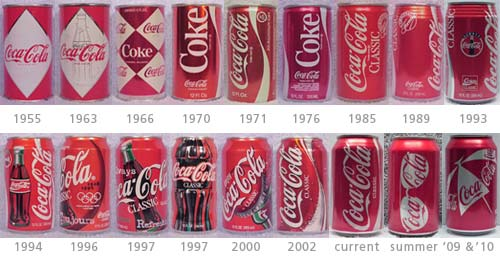
\includegraphics[width=120mm]{medias/evolution_coca}
\decoRule
\caption{Évolution du style des canettes au fil des années}
\end{figure}


\newpage


\begin{flushright}
Analyse faite par ---\\
GERARD Alexandre: \href{https://agerard57.github.io/}{https://agerard57.github.io/}\\
Mail: \href{mailto:agerard57@protonmail.com}{agerard57@protonmail.com}
\end{flushright}
